\part{Modelo Escala}

\section{Teoria}

\subsection{Escalamiento}
El análisis dimensional se utiliza para estudiar cómo cambian las fuerzas y el flujo al escalar un sistema como una ataguía. Se utilizan grupos adimensionales como el número de Reynolds, Froude y Euler.

\subsubsection{Número de Reynolds}
El número de Reynolds nos indica si el flujo es laminar o turbulento. Se calcula como:

\begin{equation}
Re = \frac{\rho V L}{\mu}
\end{equation}

Donde:
\begin{itemize}
    \item $\rho$ es la densidad del fluido,
    \item $V$ es la velocidad del agua,
    \item $L$ es la altura de la ataguía,
    \item $\mu$ es la viscosidad del agua.
\end{itemize}

Un $Re$ alto indica flujo turbulento y uno bajo flujo laminar.

\subsubsection{Número de Froude}
El número de Froude es importante cuando hay una superficie libre en el agua. Se calcula como:

\begin{equation}
Fr = \frac{V}{\sqrt{g L}}
\end{equation}

Donde:
\begin{itemize}
    \item $V$ es la velocidad del flujo,
    \item $g$ es la aceleración de la gravedad,
    \item $L$ es la altura de la ataguía.
\end{itemize}

Mantener el número de Froude constante ayuda a asegurar que el flujo tenga un comportamiento similar en un modelo a escala.

\subsubsection{Número de Euler}
El número de Euler describe la relación entre la presión y las fuerzas inerciales:

\begin{equation}
Eu = \frac{P}{\rho V^2}
\end{equation}

Donde:
\begin{itemize}
    \item $P$ es la presión ejercida por el agua,
    \item $\rho$ es la densidad del agua,
    \item $V$ es la velocidad del agua.
\end{itemize}

\subsection{Fuerza Hidrostática}
La fuerza que ejerce el agua sobre la ataguía depende de la altura del agua. La fuerza hidrostática se calcula como:

\begin{equation}
F_h = \frac{1}{2} \rho g h^2 L
\end{equation}

Donde:
\begin{itemize}
    \item $h$ es la altura del agua contra la ataguía,
    \item $L$ es la longitud de la ataguía.
\end{itemize}

Esta fuerza aumenta con el cuadrado de la altura del agua.

\subsection{Similitud en el Escalamiento}
Para que un modelo a escala sea válido, se deben cumplir tres tipos de similitud:

\begin{itemize}
    \item \textbf{Similitud geométrica}: Las dimensiones del modelo deben ser proporcionales a las del prototipo real.
    \item \textbf{Similitud cinemática}: El patrón de movimiento del agua debe ser igual en el modelo y en el sistema real, lo que se asegura manteniendo constante el número de Froude.
    \item \textbf{Similitud dinámica}: Las fuerzas que actúan deben ser proporcionales, lo que se logra manteniendo constantes números como $Re$ y $Eu$.
\end{itemize}

\subsection{Teorema de Buckingham $\pi$}

El teorema de Buckingham $\pi$ es un metodo para el análisis dimensional. Nos permite simplificar un sistema físico reduciendo sus variables dimensionales a un conjunto menor de grupos adimensionales $\pi$. Si un sistema tiene $n$ variables dimensionales y $k$ dimensiones fundamentales (como longitud, masa, y tiempo), entonces el número de grupos adimensionales es $n - k$.

Para comenzar se debe encintrar una relación funcional entre las $n$ variables dimensionales:

\begin{equation}
f(x_1, x_2, \ldots, x_n) = 0
\end{equation}

Según el teorema, esta relación puede reescribirse en términos de $n - k$ grupos adimensionales:

\begin{equation}
\pi_1 = \phi(\pi_2, \pi_3, \ldots, \pi_{n-k})
\end{equation}

Cada grupo $\pi$ es una combinación de las variables dimensionales del sistema, ajustadas para que el resultado sea adimensional. Los grupos $\pi$ tienen la forma general:

\begin{equation}
\pi_1 = x_1^{a_1} x_2^{a_2} \ldots x_n^{a_n}
\end{equation}

Los exponentes $a_1$, $a_2$, \ldots, $a_n$ se seleccionan de manera que las dimensiones de las variables se cancelen, haciendo que $\pi_1$ sea adimensional. El teorema asegura que cualquier relación física entre las variables dimensionales puede expresarse mediante estos grupos $\pi$, lo que facilita la simplificación y escalamiento de problemas físicos.

\subsection{Permeabilidad Muestra de Suelo}

Se define como permeabilidad aquella caracteristica del suelo que permite el paso del agua a travez de el \textbf{\cite{permeabilidad_suelos}}. Su unidades de medida son en Distancia/Tiemo donde existen diversas formas de estimar este coeficiente. En el caso de este proyecto, se midio un caudal con un gradiente hidraulico variable:

\begin{equation}
    k = \frac{a \cdot L}{A \cdot \Delta t} \cdot In(\frac{h1}{h2})
\end{equation}

Donde 

\section{Resultados}

\subsection{Calculo Permeabilidad Muestra}

\subsection{Licuefaccion}

A continuacion se presenta un video (ver en Adobe Acrobat) de la falla observada por licuefaccion en la maqueta a escala.

\begin{center}
    \includemedia[
        width=0.5625\textwidth, % Relación de aspecto 9:16 (altura mayor que el ancho)
        height=\textwidth,
        activate=onclick,
        addresource=VIDEOS/licuefaccion.mp4,
        flashvars={
            source=VIDEOS/licuefaccion.mp4
        }
    ]{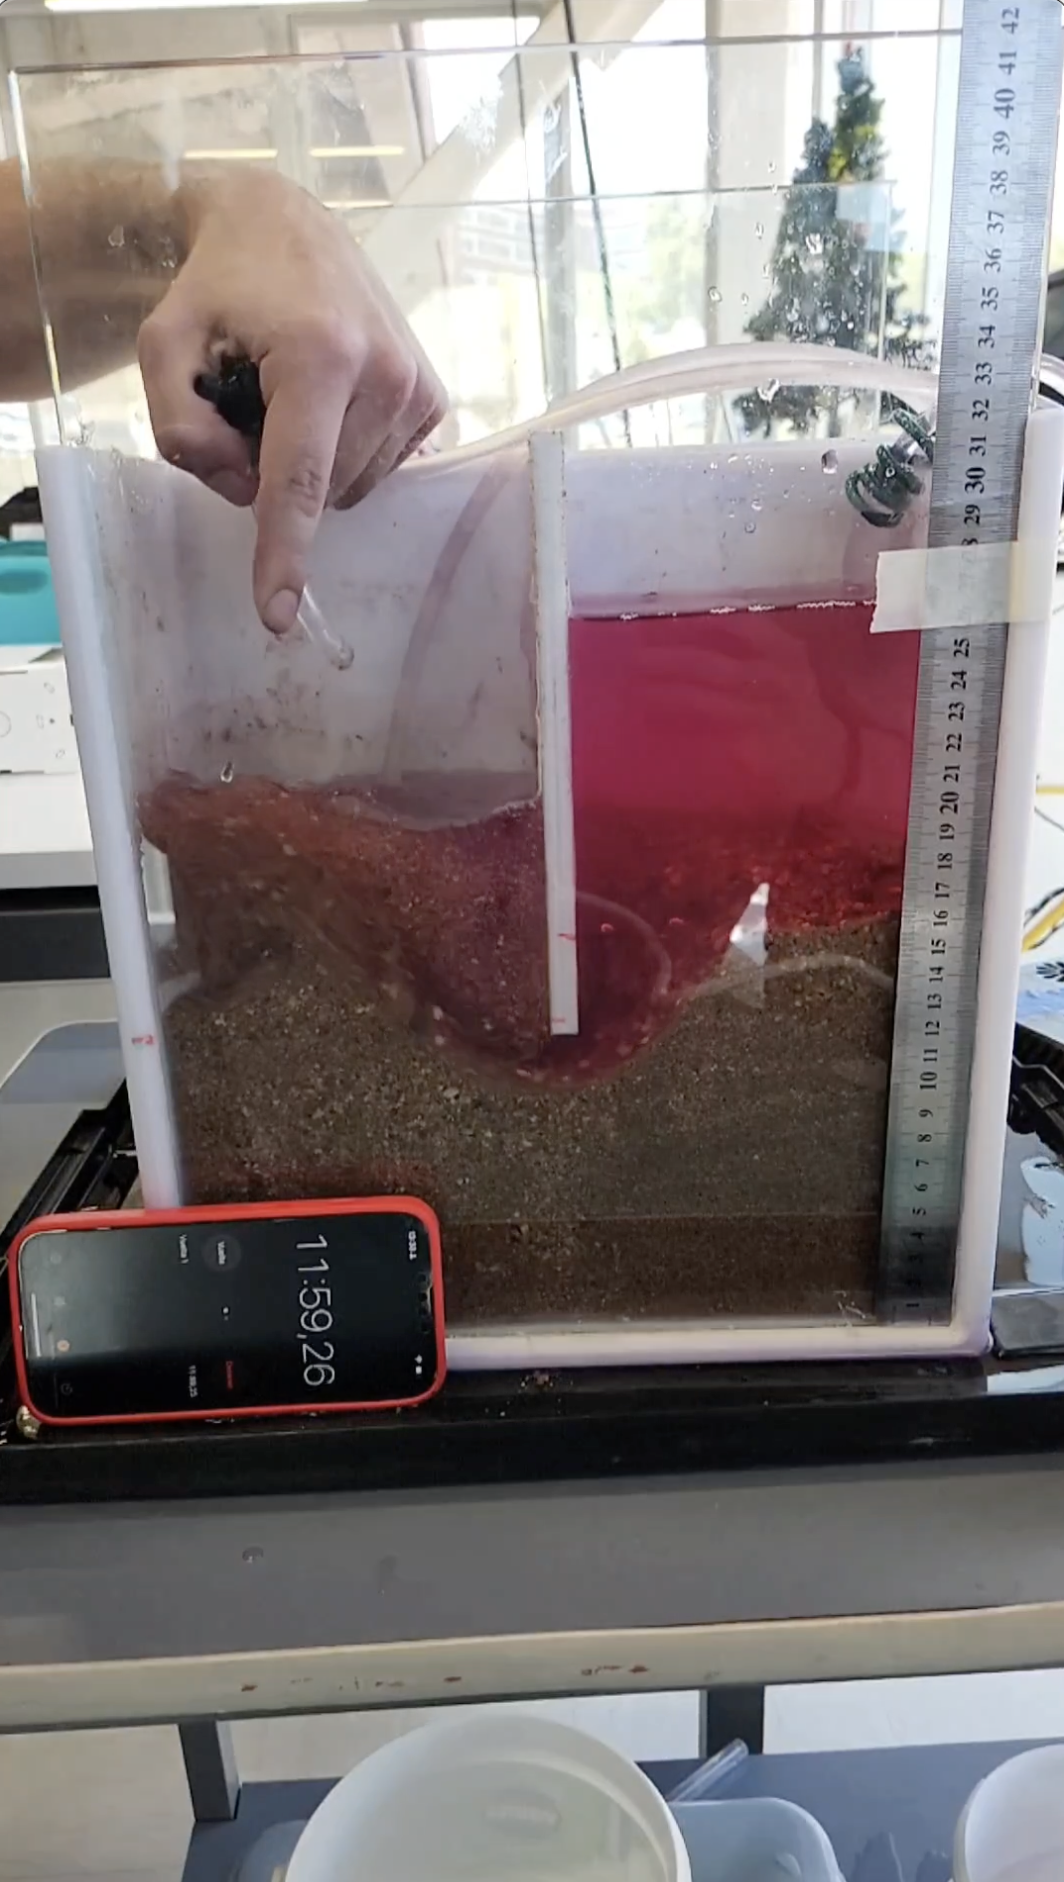
\includegraphics[width=\textwidth]{VIDEOS/miniatura_licuefaccion.png}}{VPlayer.swf}
\end{center}

Las medidas registradas son las siguientes:

\begin{table}[H]
    \centering
    \begin{tabular}{|c|c|c|c|c|c|c|c|}
    \hline
    Caso & $a_1$ & $b_1$ & $c_1$ & $a_2$ & $b_2$ & $c_2$ & $d$ \\ \hline
    Licuefaccion    & 0.0   & 14.5   & 15.5  & 15  & 2.5   & 12.5  & 0.5 \\ \hline
    \end{tabular}
    \caption{Medidas para la Licuefaccion [cm]}
    \label{tab:medidas1}
\end{table}
    

Posteriormente se realizo un mapa de calor correspondiente a la presion de poros en la licuefaccion:

\begin{figure}[H]
    \centering
    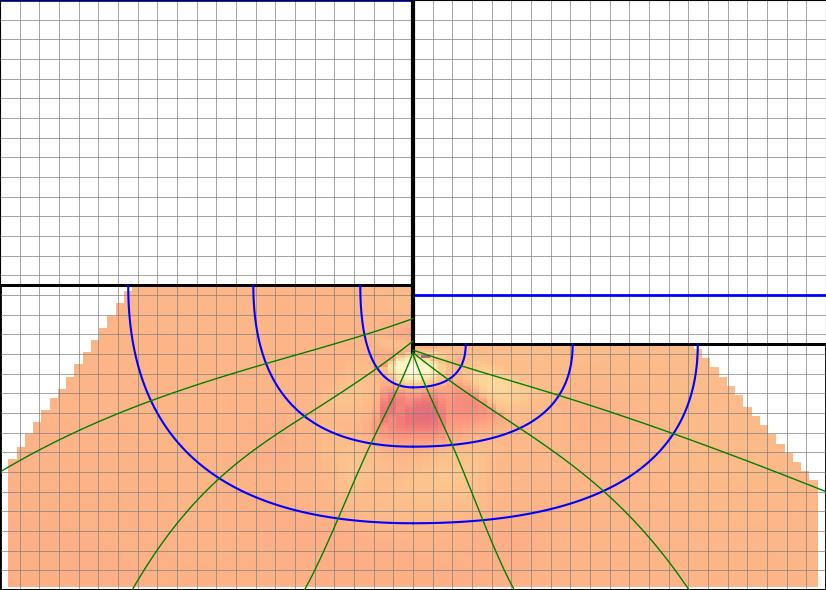
\includegraphics[width=0.5\textwidth]{GRAFICOS/caso_licuefaccion_presion_poros.jpg}
    \caption{Mapa de Calor Licuefaccion}
    \label{fig:maqueta_licuefaccion}
\end{figure}

Es interesante notar como se produce un gran aumento de presion bajo la ataguia, lo cual se observa en el video, ya que ese es el punto esperado de falla.
\\ \\
Ademas, se calculo el mismo caso segun diferencias finitas:

\begin{figure}[H]
    \centering
    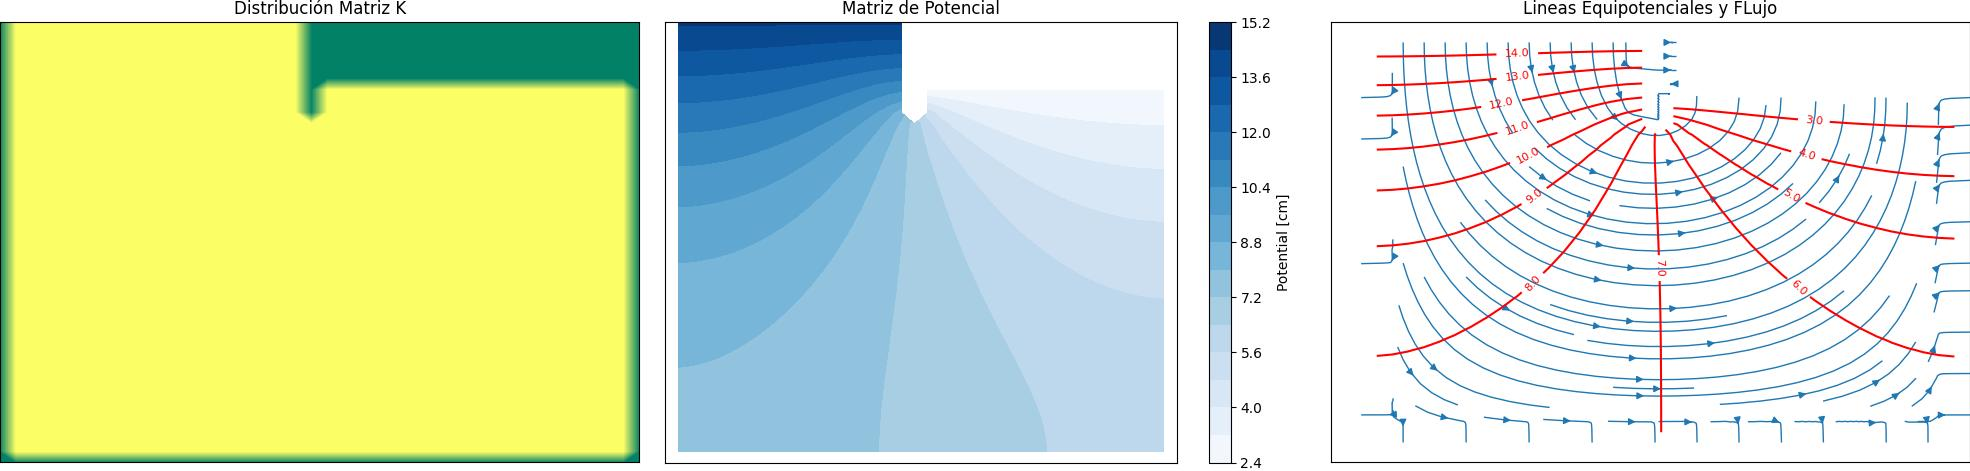
\includegraphics[width=1\textwidth]{GRAFICOS/laplace_caso_licuefaccion_escala_cm.jpg}
    \caption{Laplace Caso Licuefaccion}
    \label{fig:maqueta_licuefaccion_diferencias_finitas}
\end{figure}

\subsection{Aplicacion Diferencias Finitas}

Se determina un caudal de 0.008972885614821659 cm/s

\subsection{Caudal escalado}

Mediante la confirmacion del teorema de Buckingham $\pi$ se obtiene que el caudal del modelo es:

\begin{equation}
    Q_{modelo} = Q_{prototopo} \cdot 1.5012 \cdot 10^{-5}
\end{equation}